\documentclass{article}
\usepackage{amsmath}
\usepackage{amssymb}
\usepackage[margin=1cm,footskip=0.25cm]{geometry}
\usepackage{graphicx}
\usepackage{float}
\usepackage{multirow} % Added for multirow cells in tables
\usepackage{adjustbox} % Added for resizing tables

\begin{document}
\begin{center}
\textbf{\LARGE Lineare Algebra}
\end{center}

\section*{Matrizen}
\begin{minipage}[t]{0.45\textwidth}
    \begin{align*}
        A &= \begin{pmatrix}
        1 & 2 & 3 \\
        4 & 5 & 6 \\
        7 & 8 & 9
        \end{pmatrix}, \quad
        B = \begin{pmatrix}
        2 & 3 & 4 \\
        5 & 6 & 7 \\
        8 & 9 & 10
        \end{pmatrix}
    \end{align*}
    \subsubsection*{Addition und Subtraktion}
    \begin{align*}
    A + B &= \begin{pmatrix}
    3 & 5 & 7 \\
    9 & 11 & 13 \\
    12 & 14 & 16
    \end{pmatrix}, \quad
    A - B = \begin{pmatrix}
    -1 & -1 & -1 \\
    -1 & -1 & -1 \\
    -1 & -1 & -1
    \end{pmatrix}
    \end{align*}

    \subsubsection*{Matrizenmultiplikation}
    \begin{figure}[H]
        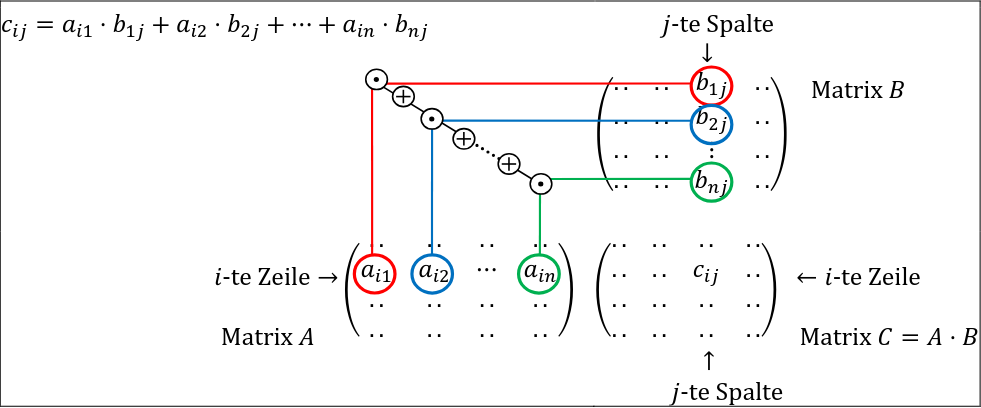
\includegraphics[scale=0.2]{images/matrixmult.png}
    \end{figure}
\end{minipage}
\hfill
\begin{minipage}[t]{0.45\textwidth}
    \subsubsection*{Transponierte Matrix}
    \begin{align*}
    A^T &= \begin{pmatrix}
    1 & 4 & 7 \\
    2 & 5 & 8 \\
    3 & 6 & 9
    \end{pmatrix}
    \end{align*}

    \subsubsection*{Multiplikation mit Skalar}
    \begin{align*}
    cA &= 2 \cdot A = \begin{pmatrix}
    2 & 4 & 6 \\
    8 & 10 & 12 \\
    14 & 16 & 18
    \end{pmatrix}
    \end{align*}
\end{minipage}

\section*{Quadratische Matrizen}
\begin{minipage}[t]{0.45\textwidth}
    \subsection*{Inverse Matrix}
    Eine Matrix \( A \) ist invertierbar / regulär, wenn es eine Matrix \( A^{-1} \) gibt, so dass \( A \cdot A^{-1} = I \), wobei \( I \) die Einheitsmatrix ist. Andernfalls ist sie singulär.
    \subsubsection*{2x2 Matrix}
    \begin{equation*}
        A = \begin{pmatrix}
        a & b \\
        c & d
        \end{pmatrix}, \quad
        A^{-1} = \frac{1}{ad - bc} \begin{pmatrix}
        d & -b \\
        -c & a
        \end{pmatrix}
    \end{equation*}
    \subsubsection*{Restliche Matrizen}
    Eine Matrix \( A \) ist invertierbar, wenn ihr Determinant \( \det(A) \neq 0 \). Die Inverse kann mit dem Gauß-Jordan-Verfahren oder der adjungierten Matrix gefunden werden.
    
    \subsection*{Eigenschaften der Determinanten}
    \begin{itemize}
        \item \( \det(A^T) = \det(A) \)
        \item \( \det(cA) = c^n \cdot \det(A) \) (für eine \( n \times n \) Matrix)
        \item \( \det(AB) = \det(A) \cdot \det(B) \)
        \item \( \det(A^{-1}) = \frac{1}{\det(A)} \)
        \item \( \det(A + B) \neq \det(A) + \det(B) \) (im Allgemeinen)
        \item \( \det(A) = 0 \) wenn \( A \) singulär ist (d.h. nicht invertierbar).
        \item Höhe des Spans: $h = \frac{|\vec{a} \cdot (\vec{b} \times \vec{c})|}{|\vec{b} \times \vec{c}|}$
    \end{itemize}
\end{minipage}
\hfill
\begin{minipage}[t]{0.45\textwidth}
    \subsection*{Determinante}
    Die Determinante einer Matrix \( A \) ist ein Skalar. Sie gibt an, ob die Matrix invertierbar ist und beschreibt das Volumen des von den Spaltenvektoren aufgespannten Parallelepipeds.
    \subsubsection*{2x2 Matrix und 3x3 Matrix}
     \begin{figure}[H]
        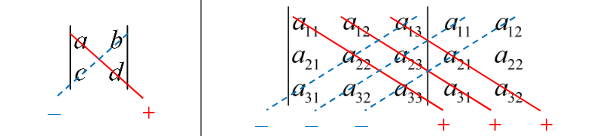
\includegraphics[scale=0.4]{images/determinante.png}
     \end{figure}

    \subsection*{Allgemeine $n \times n$-Matrix}
    Die Determinante einer \( n \times n \) Matrix kann durch Laplace-Entwicklung (für \( n > 3 \)) berechnet werden.
    
    
    \resizebox{\textwidth}{!}{%
    \begin{tabular}{|c|c|}
        \hline
        \textbf{Entwicklung nach der i-ten Zeile} & \textbf{Entwicklung nach der j-ten Spalte} \\
        \hline
        $\det(A) = \sum_{j=1}^{n} (-1)^{i+j} a_{ij} \det(A_{ij})$ 
        &
        $\det(A) = \sum_{i=1}^{n} (-1)^{i+j} a_{ij} \det(A_{ij})$
        \\
        \hline
    \end{tabular}
    }
    Die folgenden Aussagen sind äquivalent:
    \begin{itemize}
        \item $det(A) \neq 0$ 
        \item Die Spaltenvektoren von $A$ sind linear unabhängig.
        \item Die Zeilenvektoren von $A$ sind linear unabhängig.
        \item $rg(A) = n$
        \item $A$ ist invertierbar.
        \item Das LGS $A \cdot \vec{x} = \vec{b}$ hat eine eindeutige Lösung.
    \end{itemize}
\end{minipage}

\section*{Lineare Gleichungssysteme}
\begin{minipage}[t]{0.45\textwidth}
    \subsection*{Zeilenstufenform}
    Die Matrix ist in Zeilenstufenform, wenn:
    \begin{itemize}
        \item Alle Zeilen, die nur Nullen enthalten, stehen am Ende der Matrix.
        \item Die erste Nicht-Null-Zahl in jeder Zeile (der sogenannte Pivot) ist 1 (führende Eins).
        \item Der Pivot jeder Zeile steht weiter rechts als der Pivot der vorherigen Zeile.
    \end{itemize}
    Reduzierte Zeilenstufenform (RREF) ist erreicht, wenn:
    \begin{itemize}
        \item Jede Spalte, die eine führende Eins enthält, hat nur Nullen in allen anderen Zeilen.
    \end{itemize}    
\end{minipage}
\hfill
\begin{minipage}[t]{0.45\textwidth}
    \subsection*{Parameterdarstellung}
    \subsubsection*{führende Unbekannte}
    Die führenden Unbekannten sind die Variablen, die in der Zeilenstufenform der Matrix als Pivot-Elemente auftreten. Sie sind eindeutig bestimmt und können direkt aus den Gleichungen abgelesen werden.
    \subsubsection*{freie Unbekannte}
    Die freien Unbekannten sind die Variablen, die nicht als Pivot-Elemente auftreten. Sie können beliebige Werte annehmen.
    
\end{minipage}
\subsubsection*{Beispiel}
\begin{align*}
    \begin{pmatrix}
    1 & -2 & 0 & 3 | 5 \\
    0 & 0 & 1 & 1 | 3
    \end{pmatrix}
\end{align*}
In diesem Beispiel sind $x_1$ und $x_3$ die führenden Unbekannten, während $x_2$ und $x_34$ freie Unbekannte sind. Die Lösung kann in Parameterform dargestellt werden:

\begin{minipage}[t]{0.45\textwidth}
    \begin{align*}
        x_2 &= \lambda \quad (\lambda \in \mathbb{R}) \\
        x_4 &= \mu \quad (\mu \in \mathbb{R})
    \end{align*}
    Erste Zeile: \( x_1 - 2x_2 + 3x_4 = 5 \), daraus \( x_1 = 5 + 2\lambda - 3\mu \)\\
    Zweite Zeile: \( x_3 + x_4 = 3 \), daraus \( x_3 = 3 - \mu \)
\end{minipage}
\hfill
\begin{minipage}[t]{0.45\textwidth}
    In Vektorform:

    \begin{align*}
        \begin{pmatrix}
        x_1 \\
        x_2 \\
        x_3 \\
        x_4
        \end{pmatrix}
        = 
        \begin{pmatrix}
        5 \\
        0 \\
        3 \\
        0
        \end{pmatrix}
        + \lambda
        \begin{pmatrix}
        2 \\
        1 \\
        0 \\
        0
        \end{pmatrix}
        + \mu
        \begin{pmatrix}
            -3 \\
            0 \\
            -1 \\
            1
        \end{pmatrix}
    \end{align*}
\end{minipage}

\section*{Lösbarkeit von LGS}
\begin{itemize}
    \item \textbf{Eindeutige Lösung:} Wenn die Matrix in Zeilenstufenform keine freien Unbekannten hat. (rg(A) = Anzahl der Unbekannten (n))
    \item \textbf{Unendlich viele Lösungen:} Wenn die Matrix in Zeilenstufenform mindestens eine freie Unbekannte hat. ($rg(A) <  n$)
    \item \textbf{Keine Lösung:} Wenn die Matrix in Zeilenstufenform eine Zeile der Form \(0 = c\) (mit \(c \neq 0\)) enthält. ($rg(A) \neq rg(A|\vec{c})$)
\end{itemize}

\section*{Vektorgeometrie}
\begin{minipage}[t]{0.45\textwidth}
    \subsection*{Einheitsvektor}
    Ein Einheitsvektor ist ein Vektor mit der Länge/Betrag 1.

    \subsection*{Koliniare Vektoren}
    Zwei Vektoren \( \vec{a} \) und \( \vec{b} \) sind kolinear, wenn sie in die gleiche Richtung zeigen oder entgegengesetzt sind, bzw. das Vektorprodukt 0 ergibt. Mathematisch ausgedrückt: \( \vec{a} = k \cdot \vec{b} \) für ein Skalar \( k \).
    Der Nullvektor ist kolinear zu jedem Vektor. \( \vec{a} \times \vec{b} = \vec{0} \)

    \subsection*{Komplanare Vektoren}
    Drei Vektoren \( \vec{a}, \vec{b}, \vec{c} \) sind komplanar, wenn sie in einer Ebene liegen. Dies ist der Fall, wenn das Skalarprodukt der Kreuzprodukte Null ist: \( \vec{a} \times \vec{b} \cdot \vec{c} = 0 \).

    \subsection*{Orthogonale Projektion}
    Die orthogonale Projektion eines Vektors \( \vec{a} \) auf einen Vektor \( \vec{b} \) wird berechnet als:
    \begin{equation*}
        \vec{b}_{\vec{a}} = \frac{\vec{a} \cdot \vec{b}}{|\vec{a}|^2} \cdot \vec{a} 
        \quad \Leftrightarrow \quad 
        |\vec{b}_{\vec{a}}| = \frac{|\vec{a} \cdot \vec{b}|}{|\vec{a}|}
    \end{equation*}
    Die Projektion gibt den Anteil von \( \vec{a} \) in Richtung von \( \vec{b} \) an.

    \subsection*{Vektorprodukt}
    Das Vektorprodukt (Kreuzprodukt) zweier Vektoren \( \vec{a} = (a_1, a_2, a_3) \) und \( \vec{b} = (b_1, b_2, b_3) \) wird berechnet als:
    \begin{equation*}
    \vec{a} \times \vec{b} = 
    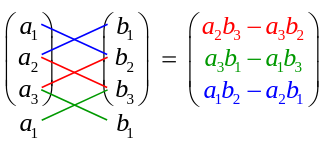
\includegraphics[scale=0.3]{images/vektorprodukt.png}
    \end{equation*}
    \begin{equation*}
        |\vec{a} \times \vec{b}| = |\vec{a}| \cdot |\vec{b}| \cdot \sin(\theta)
    \end{equation*}
    Das Vektorprodukt ist ein Vektor, der orthogonal zu beiden Ausgangsvektoren steht. Die Länge des Vektorprodukts entspricht der Fläche des Parallelogramms, das von den beiden Vektoren aufgespannt wird.

    \subsubsection*{Eigenschaften des Vektorprodukts}
    \begin{itemize}
        \item \( \vec{a} \times \vec{b} = -(\vec{b} \times \vec{a}) \) (Antisymmetrie)
        \item Distributivität: \( \vec{a} \times (\vec{b} + \vec{c}) = \vec{a} \times \vec{b} + \vec{a} \times \vec{c} \)
        \item Gemischtes Assoziativ-Gesetz: \( \lambda \cdot (\vec{a} \times \vec{b}) = (\lambda \cdot \vec{a}) \times \vec{b} = \vec{a} \times (\lambda \cdot \vec{b}) \)
    \end{itemize}
\end{minipage}
\hfill
\begin{minipage}[t]{0.45\textwidth}
    \subsection*{Betrag eines Vektors}
    Der Betrag eines Vektors \( \vec{a} = (a_1, a_2, a_3) \) wird berechnet als:
    \begin{equation*}
        |\vec{a}| = \sqrt{a_1^2 + a_2^2 + a_3^2}
    \end{equation*}


    \subsection*{Basisvektoren}
    Eine Basis eines Vektorraums ist eine Menge von Vektoren, die linear unabhängig sind und den gesamten Raum aufspannen. Jeder Vektor im Raum kann als Linearkombination dieser Basisvektoren dargestellt werden.
    
    \subsection*{Skalarprodukt}
    Das Skalarprodukt zweier Vektoren \( \vec{a} = (a_1, a_2, a_3) \) und \( \vec{b} = (b_1, b_2, b_3) \) wird berechnet als:
    \begin{equation*}
        \vec{a} \cdot \vec{b} = a_1 b_1 + a_2 b_2 + a_3 b_3
    \end{equation*}
    Das Skalarprodukt ist ein Maß für die Ähnlichkeit zweier Vektoren. Es ist null, wenn die Vektoren orthogonal zueinander sind.
    \subsection*{Winkel zwischen Vektoren}
    Der Winkel \( \theta \) zwischen zwei Vektoren \( \vec{a} \) und \( \vec{b} \) kann mit dem Skalarprodukt berechnet werden:
    \begin{equation*}
        \cos(\theta) = \frac{\vec{a} \cdot \vec{b}}{|\vec{a}| |\vec{b}|} 
        \quad \Leftrightarrow \quad 
        \theta = \arccos\left(\frac{\vec{a} \cdot \vec{b}}{|\vec{a}| |\vec{b}|}\right) 
    \end{equation*}

    \subsection*{Gegenseitige Lage von Geraden im Raum}
    \begin{center}
    \resizebox{\textwidth}{!}{%
    \begin{tabular}{|l|l|l|l|}
    \hline
    \multicolumn{2}{|c|}{} & \multicolumn{2}{c|}{Gibt es einen gemeinsamen Punkt?} \\
    \cline{3-4}
    \multicolumn{2}{|c|}{} & ja & nein \\
    \hline
    \multirow{2}{*}{Sind die Richtungsvektoren kollinear?} & ja & identisch & echt parallel \\
    \cline{2-4}
    & nein & schneidend & windschief \\
    \hline
    \end{tabular}%
    }
    \end{center}
    \subsection*{Abstand zwischen einer Geraden und einem Punkt}
    Der Abstand \( d \) zwischen einer Geraden \( g \) und einem Punkt \( P \) kann mithilfe der Fläche des Parallelogramms berechnet werden, 
    das von den Richtungsvektoren der Geraden und dem Vektor vom Punkt auf die Gerade aufgespannt wird:
    \begin{equation*}
        \overrightarrow{PA} = \vec{P} - \vec{A}
    \end{equation*}
    \begin{equation*}
        F = |\overrightarrow{PA} \times \vec{a}|
        \quad \text{(Fläche des Parallelogramms)}
    \end{equation*}
    \begin{equation*}
        l = \frac{F}{|\vec{a}|}
        \quad \text{(Länge der Geraden)}
    \end{equation*}
\end{minipage}

\begin{minipage}[t]{0.45\textwidth}
    \subsection*{Koordinatendarstellung von Geraden in der Ebene}
    Eine Gerade in der Ebene kann durch die Gleichung
    \begin{equation*}
        g: ax + by + c = 0
    \end{equation*}
    dargestellt werden.
    \subsubsection*{Umrechnung Parameterdarstellung $\to$ Koordinatendarstellung}
    \begin{equation*}
        \vec{r}(A) = \begin{pmatrix}
        x \\
        y
        \end{pmatrix} = \vec{r}(P) + \lambda \cdot \vec{a}
    \end{equation*}
    Daraus lässt sich ein Gleichungssystem ableiten
\end{minipage}
\hfill
\begin{minipage}[t]{0.45\textwidth}
    \subsubsection*{Umrechnung Koordinatendarstellung $\to$ Parameterdarstellung}
    Wir bestimmen zwei beliebige Punkte auf $g$, indem wir die $x$-Koordinaten frei wählen und die
zugehörigen $y$-Koordinaten aus der Koordinatendarstellung von $g$ berechnen. Aus diesen beiden
Punkten können wir dann eine Parameterdarstellung von $g$ gewinnen.
\end{minipage}

\section*{Ebenen}
\begin{minipage}[t]{0.45\textwidth}
    \subsection*{Parameterdarstellung}
    Eine Ebene im Raum kann durch die Gleichung
    \begin{equation*}
        E: \vec{r}(P) + \lambda_1 \cdot \vec{a} + \lambda_2 \cdot \vec{b}
    \end{equation*}
    dargestellt werden, wobei \( \vec{r}(P) \) ein Punkt auf der Ebene ist und \( \vec{a} \) und \( \vec{b} \) zwei Richtungsvektoren der Ebene sind.
    \subsection*{Koordinatendarstellung}
    Eine Ebene kann auch in der Koordinatendarstellung angegeben werden:
    \begin{equation*}
        E: ax + by + cz + d = 0
    \end{equation*}
    Hierbei sind \( a, b, c \) die Komponenten des Normalenvektors der Ebene und \( d \) eine Konstante.

    \subsection*{Abstand zwischen einer Ebene und einem Punkt}
    Um den Abstand $l$ zu berechnen, gehen wir folgendermassen vor:
    Wir wählen einen beliebigen Punkt $P$ der Ebene $E$ (rechts "im
    Profil" abgebildet). Dann projizieren wir den Verbindungsvektor
    $\overrightarrow{PA}$ auf den Normalenvektor $\vec{n}$ der Ebene. Die Länge dieser
    Projektion ist gerade der gesuchte Abstand $l$.
    \begin{equation*}
        l = \frac{|ax_A + by_A + cz_A + d|}{|\vec{n}|}
    \end{equation*}
\end{minipage}
\hfill
\begin{minipage}[t]{0.45\textwidth}
    \subsection*{Schnittpunkt Ebene und Gerade}
    Der Schnittpunkt einer Ebene \( E \) und einer Geraden \( g \) kann mithilfe eines LGS gefunden werden. 
    \begin{equation*}
        E: \begin{pmatrix}
            1 \\
            0 \\
            -2
        \end{pmatrix} + \lambda \cdot \begin{pmatrix}
            3 \\
            -2 \\
            1
        \end{pmatrix} + \mu \cdot \begin{pmatrix}
            0 \\
            4 \\
            3
        \end{pmatrix}
    \end{equation*}
    \begin{equation*}
        g: \begin{pmatrix}
            1 \\
            -3 \\
            -4
            \end{pmatrix} + v \cdot \begin{pmatrix}
                -2 \\
                1 \\
                -1
            \end{pmatrix}
    \end{equation*}
    Um den Schnittpunkt zu finden, setzen wir die Ebene und die Gerade gleich und lösen das entstehende LGS

    \subsection*{Gegenseitige Lage von Ebenen}
    \subsubsection*{identisch}
    Zwei Ebenen sind identisch, wenn sie die gleiche Normalenvektor und den gleichen Stützpunkt haben.

    \subsubsection*{echt parallel}
    Zwei Ebenen sind echt parallel, wenn ihre Normalenvektoren kollinear sind, aber sie nicht identisch sind.
    
    \subsubsection*{schneidend}
    In allen anderen Fällen schneiden sich die Ebenen. Der Schnittpunkt kann durch das Lösen eines LGS gefunden werden.
\end{minipage}

\section*{Reeler Vektorraum}
\begin{minipage}[t]{0.45\textwidth}
    \subsection*{Definition}
    Ein reeller Vektorraum ist eine Menge von Vektoren, die unter Addition und Skalarmultiplikation abgeschlossen ist. 
    Die Vektoren können addiert und mit reellen Zahlen skaliert werden, wobei die folgenden Axiome erfüllt sein müssen:
    \begin{itemize}
        \item Assoziativität der Addition
        \item Kommutativität der Addition
        \item Existenz eines Nullvektors
        \item Existenz eines inversen Vektors
        \item Distributivität der Skalarmultiplikation
        \item Assoziativität der Skalarmultiplikation
        \item Identitätselement der Skalarmultiplikation
        \item Wenn ich 2 Elemente in V addiere, muss das Ergebnis auch in V sein.
        \item Wenn ich ein Element in V mit einem Skalar multipliziere, muss das Ergebnis auch in V sein.
    \end{itemize}

    \subsection*{Umrechnung von Komponentendarstellungen}
    \subsubsection*{Basis $\mathcal{B} \to$ Basis $\mathcal{S}$}
    Um von einer Basis \( \mathcal{B} \)  zu einer Basis \( \mathcal{S} \) zu wechseln, verwenden wir die Umrechnungsformel:
    \begin{equation*}
        \vec{a}_{\mathcal{S}} = v_1 \cdot \vec{b}_1 + v_2 \cdot \vec{b}_2 + \ldots + v_n \cdot \vec{b}_n
    % \end{pmatrix} 
    \end{equation*}
    $b_{1 \ldots b_n}$ sind die Basisvektoren der Basis $\mathcal{B}$, $v_1 \ldots v_n$ sind die Komponenten des Vektors in der Basis $\mathcal{B}$.

    \subsubsection*{Basis $\mathcal{S} \to$ Basis $\mathcal{B}$}
    Um von einer Basis \( \mathcal{S} \) zu einer Basis \( \mathcal{B} \) zu wechseln, nutzen wir ein LGS:
    \begin{equation*}
        \vec{a}_{\mathcal{B}} = w_1 \cdot \vec{s}_1 + w_2 \cdot \vec{s}_2 + \ldots + w_n \cdot \vec{s}_n
    \end{equation*}
    $s_{1 \ldots s_n}$ sind die Basisvektoren der Basis $\mathcal{B}$, $w_1 \ldots w_n$ sind die Komponenten des Vektors in der Basis $\mathcal{S}$.

\end{minipage}
\hfill
\begin{minipage}[t]{0.45\textwidth}
    \subsection*{Unterräume}
    Ein Unterraum eines Vektorraums ist eine Teilmenge, die selbst ein Vektorraum ist. Er muss die Null enthalten und abgeschlossen unter Addition und Skalarmultiplikation sein.
    
    \subsection*{Basis und Dimension}
    Eine Basis eines Vektorraums ist eine Menge von linear unabhängigen Vektoren, die den gesamten Raum aufspannen. Die Dimension des Vektorraums ist die Anzahl der Vektoren in einer Basis.

    \subsection*{Erzegendensyteme}
    Ein Erzeugendensystem eines Vektorraums ist eine Menge von Vektoren, deren Linearkombinationen den gesamten Raum aufspannen. Es kann mehr Vektoren enthalten als eine Basis, aber nicht weniger.
    
    Die folgenden Aussagen sind äquivalent:
    \begin{itemize}
        \item Die Vektoren $b_1, b_2, \ldots, b_n$ bilden ein Erzeugendensystem von $\mathbb{R}^n$.
        \item Das LGS $A \cdot \vec{x} = \vec{b}$ hat für jedes $\vec{b} \in \mathbb{R}^n$ eine Lösung.
        \item Die Matrix $A$ hat vollen Rang, d.h. $rg(A) = n$.
    \end{itemize}

    \subsection*{Lineare Unabhängigkeit}
    Eine Menge von Vektoren \( \vec{v}_1, \vec{v}_2, \ldots, \vec{v}_n \) ist linear unabhängig, wenn die Gleichung
    \begin{equation*}
        c_1 \vec{v}_1 + c_2 \vec{v}_2 + \ldots + c_n \vec{v}_n = 0
    \end{equation*}
    nur die triviale Lösung \( c_1 = c_2 = \ldots = c_n = 0 \) hat. Andernfalls sind die Vektoren linear abhängig.
\end{minipage}

\pagebreak

\section*{Lineare Abbildungen}
\begin{minipage}[t]{0.45\textwidth}
    \subsection*{Definition}
    Eine lineare Abbildung \( f: V \to W \) zwischen zwei Vektorräumen \( V \) und \( W \) ist eine Funktion, die die folgenden Eigenschaften erfüllt:
    \begin{itemize}
        \item \( f(\vec{u} + \vec{v}) = f(\vec{u}) + f(\vec{v}) \) für alle \( \vec{u}, \vec{v} \in V \)
        \item $\lambda \cdot \vec{v} = \lambda \cdot f(\vec{v})$ für alle \( c \in \mathbb{R} \) und \( \vec{v} \in V \)
    \end{itemize}

    \subsection*{Kern und Bild}
    Der Kern \( \ker(f) \) einer linearen Abbildung \( f \) ist die Menge aller Vektoren \( \vec{v} \in V \), für die \( f(\vec{v}) = \vec{0} \). (z-Achse)
    
    Das Bild \( \text{Im}(f) \) ist die Menge aller Vektoren \( \vec{w} \in W \), die als Bild eines Vektors aus \( V \) unter \( f \) entstehen, d.h. \( \text{Im}(f) = \{ f(\vec{v}) | \vec{v} \in V \} \). (xy-Ebene)
    \newline
    \newline
    \textbf{$m \times n$ Matrix $f$ }
    \begin{equation*}
        dim(ker(f)) + dim(Im(f)) = n
    \end{equation*}

    \subsection*{Basenwechsel}
    Wenn \( \mathcal{B} \) eine Basis von \( V \) und \( \mathcal{S} \) eine Basis von \( W \) ist, dann kann die lineare Abbildung \( f \) in Bezug auf diese Basen dargestellt werden.

    \subsubsection*{$\mathcal{B} \to \mathcal{S}$}
    Um die Abbildung \( f \) von der Basis \( \mathcal{B} \) zu \( \mathcal{S} \) zu beschreiben, verwenden wir die Abbildungsmatrix \( A \):
    \begin{equation*}
        {}_{\mathcal{S}}T_{\mathcal{B}} = \begin{pmatrix}
            | & | & & | \\
            f(\vec{b}_1)_{\mathcal{S}} & f(\vec{b}_2)_{\mathcal{S}} & \ldots & f(\vec{b}_n)_{\mathcal{S}} \\
            | & | & & |
        \end{pmatrix}
    \end{equation*}

    \subsubsection*{$\mathcal{S} \to \mathcal{B}$}
    Das ist die Inverse Abbildung, die die Abbildung von der Basis \( \mathcal{S} \) zurück zur Basis \( \mathcal{B} \) beschreibt. Sie wird ebenfalls durch eine Matrix \( B \) dargestellt:
    \begin{equation*}
        {}_{\mathcal{B}}T_{\mathcal{S}} = {}_{\mathcal{S}}T_{\mathcal{B}}^{-1}
    \end{equation*}

\end{minipage}
\hfill
\begin{minipage}[t]{0.45\textwidth}
    \subsection*{Abbildungsmatrix}
    Die Abbildungsmatrix \( A \) einer linearen Abbildung \( f \) bezüglich der Basen \( \mathcal{B} \) von \( V \) und \( \mathcal{S} \) von \( W \) ist die Matrix, 
    die die Abbildung \( f \) beschreibt. Sie wird gebildet, indem die Bilder der Basisvektoren von \( V \) in Bezug auf die Basis von \( W \) dargestellt werden.

    \subsection*{Verknüpfung von linearen Abbildungen}
    Wenn \( f: V \to W \) und \( g: W \to U \) zwei lineare Abbildungen sind, dann ist die Verknüpfung \( g \circ f: V \to U \) ebenfalls eine lineare Abbildung.

    \subsubsection*{Allgemein}
    Die Matrix der Abbildung die zuerst aufgeführt wird, steht rechts ($f \circ g \implies A \cdot B$).

    \subsubsection*{Spiegelung}
    $S^2 = I$ (Identitätsmatrix), da Spiegelungen ihre eigene Inverse sind.

    \subsubsection*{Projektion}
    $P^2 = P$ (Projektion ist idempotent), da eine Projektion auf einen Unterraum ihre eigene Inverse ist.

    \subsection*{Homogene Koordinaten}
    Homogene Koordinaten erweitern die üblichen Koordinaten um eine zusätzliche Dimension, um affine Abbildungen (wie Translationen) in lineare Abbildungen umzuwandeln.
    
    Es wird ein zusätzlicher Parameter \( w \) eingeführt, sodass ein Punkt \( (x, y) \) in der Ebene als \( (x, y, w) \) dargestellt wird.
\end{minipage}

\subsection*{Beispiele von linearen Abbildungen}
\begin{minipage}[t]{0.45\textwidth}
    \subsubsection*{Ebene}
    \resizebox{\textwidth}{!}{%
    \begin{tabular}{|c|c|}
        \hline
        \textbf{Abbildung} & \textbf{Matrix} \\
        \hline
        Drehung um den Ursprung & \( A = \begin{pmatrix}
        \cos(\theta) & -\sin(\theta) \\
        \sin(\theta) & \cos(\theta)
        \end{pmatrix} \) \\
        \hline
        Streckung & \( A = \begin{pmatrix}
        \lambda_1 & 0 \\
        0 & \lambda_2
        \end{pmatrix} \) \\
        \hline
        Spiegelung an der x-Achse & \( A = \begin{pmatrix}
        1 & 0 \\
        0 & -1
        \end{pmatrix} \) \\
        \hline
        Spiegelung an der y-Achse & \( A = \begin{pmatrix}
        -1 & 0 \\
        0 & 1
        \end{pmatrix} \) \\
        \hline
        Spiegelung an der Geraden \( y = x \) & \( A = \begin{pmatrix}
        0 & 1 \\
        1 & 0
        \end{pmatrix} \) \\
        \hline
        Spiegelung an der Geraden \( y = -x \) & \( A = \begin{pmatrix}
        0 & -1 \\
        -1 & 0
        \end{pmatrix} \) \\
        \hline
        Orthogonale Projektion auf die x-Achse & \( A = \begin{pmatrix}
        1 & 0 \\
        0 & 0
        \end{pmatrix} \) \\
        \hline
        Orthogonale Projektion auf die y-Achse & \( A = \begin{pmatrix}
        0 & 0 \\
        0 & 1
        \end{pmatrix} \) \\
        \hline
        Scherung in x-Richtung ($k = \tan(\theta)$) & \( A = \begin{pmatrix}
        1 & k \\
        0 & 1
        \end{pmatrix} \) \\
        \hline
    \end{tabular}
    }

    \subsubsection*{Rotation im Raum um eine allgemeine Achse durch den Ursprung}
    \resizebox{\textwidth}{!}{%
    $\begin{pmatrix}
        \cos(\theta) + n_1^2(1 - \cos(\theta)) & n_1n_2(1 - \cos(\theta)) - n_3\sin(\theta) & n_1n_3(1 - \cos(\theta)) + n_2\sin(\theta) \\
        n_2n_1(1 - \cos(\theta)) + n_3\sin(\theta) & \cos(\theta) + n_2^2(1 - \cos(\theta)) & n_2n_3(1 - \cos(\theta)) - n_1\sin(\theta) \\
        n_3n_1(1 - \cos(\theta)) - n_2\sin(\theta) & n_3n_2(1 - \cos(\theta)) + n_1\sin(\theta) & \cos(\theta) + n_3^2(1 - \cos(\theta))
    \end{pmatrix}$
    }
\end{minipage}
\hfill
\begin{minipage}[t]{0.45\textwidth}
    \subsubsection*{Raum}
    \resizebox{\textwidth}{!}{%
    \begin{tabular}{|c|c|}
        \hline
        \textbf{Abbildung} & \textbf{Matrix} \\
        \hline
        Drehung um den Ursprung & \( A = \begin{pmatrix}
        \cos(\theta) & -\sin(\theta) & 0 \\
        \sin(\theta) & \cos(\theta) & 0 \\
        0 & 0 & 1
        \end{pmatrix} \) \\
        \hline
        Streckung & \( A = \begin{pmatrix}
        \lambda_1 & 0 & 0 \\
        0 & \lambda_2 & 0 \\
        0 & 0 & \lambda_3
        \end{pmatrix} \) \\
        \hline
        Spiegelung an der xy-Ebene & \( A = \begin{pmatrix}
        1 & 0 & 0 \\
        0 & -1 & 0 \\
        0 & 0 & -1
        \end{pmatrix} \) \\
        \hline
        Spiegelung an der xz-Ebene & \( A = \begin{pmatrix}
        -1 & 0 & 0 \\
        0 & 1 & 0 \\
        0 & 0 & -1
        \end{pmatrix} \) \\
        \hline
        Spiegelung an der yz-Ebene & \( A = \begin{pmatrix}
        -1 & 0 & 0 \\
        0 & -1 & 0 \\
        0 & 0 & 1
        \end{pmatrix} \) \\
        \hline
        Scherung in x-Richtung (3D) & $A = \begin{pmatrix}
        1 & k & l \\
        0 & 1 & m \\
        0 & 0 & 1
        \end{pmatrix}$ \\
        \hline
        Scherung in y-Richtung (3D) & $A = \begin{pmatrix}
        1 & 0 & l \\
        k & 1 & m \\
        0 & 0 & 1
        \end{pmatrix}$ \\
        \hline
        Scherung in z-Richtung (3D) & $A = \begin{pmatrix}
        1 & 0 & k \\
        0 & 1 & l \\
        m & 0 & 1
        \end{pmatrix}$ \\
        \hline
        Orthogonale Projektion auf die xy-Ebene & \( A = \begin{pmatrix}
        1 & 0 & 0 \\
        0 & 1 & 0 \\
        0 & 0 & 0
        \end{pmatrix} \) \\
        \hline
        Orthogonale Projektion auf die xz-Ebene & \( A = \begin{pmatrix}
        1 & 0 & 0 \\
        0 & 0 & 0 \\
        0 & 0 & 1
        \end{pmatrix} \) \\
        \hline
        Orthogonale Projektion auf die yz-Ebene & \( A = \begin{pmatrix}
        0 & 0 & 0 \\
        0 & 1 & 0 \\
        0 & 0 & 1
        \end{pmatrix} \) \\
        \hline
        Orthogonale Projektion auf die x-Achse & \( A = \begin{pmatrix}
        1 & 0 & 0 \\
        0 & 0 & 0 \\
        0 & 0 & 0
        \end{pmatrix} \) \\
        \hline
        Orthogonale Projektion auf die y-Achse & \( A = \begin{pmatrix}
        0 & 0 & 0 \\
        0 & 1 & 0 \\
        0 & 0 & 0
        \end{pmatrix} \) \\
        \hline
        Orthogonale Projektion auf die z-Achse & \( A = \begin{pmatrix}
        0 & 0 & 0 \\
        0 & 0 & 0 \\
        0 & 0 & 1
        \end{pmatrix} \) \\
        \hline
        Spiegelung an einer allgemeinen Ebene \\ durch den Ursprung & \( A = \begin{pmatrix}
        1 - 2n_1^2 & -2n_1n_2 & -2n_1n_3 \\
        -2n_1n_2 & 1 - 2n_2^2 & -2n_2n_3 \\
        -2n_1n_3 & -2n_2n_3 & 1 - 2n_3^2
        \end{pmatrix} \) \\
        \hline
        Rotation um die z-Achse & \( A = \begin{pmatrix}
        \cos(\theta) & -\sin(\theta) & 0 \\
        \sin(\theta) & \cos(\theta) & 0 \\
        0 & 0 & 1
        \end{pmatrix} \) \\
        \hline
        Rotation um die y-Achse & \( A = \begin{pmatrix}
        \cos(\theta) & 0 & -\sin(\theta) \\
        0 & 1 & 0 \\
        \sin(\theta) & 0 & \cos(\theta)
        \end{pmatrix} \) \\
        \hline
        Rotation um die x-Achse & \( A = \begin{pmatrix}
        1 & 0 & 0 \\
        0 & \cos(\theta) & -\sin(\theta) \\
        0 & \sin(\theta) & \cos(\theta)
        \end{pmatrix} \) \\
        \hline
    \end{tabular}
    }
\end{minipage}
\end{document}